\documentclass[]{article}
\usepackage[margin=3cm]{geometry}
\usepackage{graphicx}
\usepackage{subcaption}
\usepackage{float}
\usepackage{amsmath}
\usepackage{enumerate}
\usepackage{amsmath}
\usepackage{bm}
\usepackage[linesnumbered,ruled,vlined]{algorithm2e}
% custom commands %
\newcommand{\half}{\frac{1}{2}}
\newcommand{\dd}{\textnormal{d}}
\newcommand{\ddx}{\frac{\dd}{\dd x}}
\newcommand{\dydx}{\frac{\dd y}{\dd x}}
\newcommand{\bfx}{\textbf{x}}
\newcommand{\bfR}{\textbf{R}}
%%% redefine eqnarray to not put equation numbering
\newenvironment{eq}
{\begin{eqnarray*}}
	{\end{eqnarray*}}
%%%

%opening
\title{A general simulated annealing approach to extracting nuclear dynamics from ultrafast x-ray scattering data}
\author{Thomas Northey}
\date{\today}

\begin{document}
	
	\maketitle
	
	\begin{abstract}
		abst
	\end{abstract}
	
	\section{Introduction}
	1m structure method \cite{yong2021determination}
	
	Some references \cite{yong2019scattering,yong2021determination,stankus2019ultrafast,wolf2019photochemical,moreno2019ab,northey2014ab,northey2016elastic}
	
	\subsection{Simulated annealing}
	
	Simulated annealing is a type of Metropolis algorithm, in that it always takes a downhill step while sometimes taking an uphill step \cite{press2007numerical}.
	
	It is a powerful tool in combinatorial minimisation, where the space over the which the function is defined is a discrete but very large configuration space. The size of the configurational space is factorially large, so that it cannot be explored exhaustively. Furthermore, since the set is discrete, we are deprived of any notion of continuing downhill in a favourable direction. The concept of direction may not have any meaning in the configuration space. A classic example of this is the travelling salesman problem.(taken from \cite{press2007numerical})
	
	
	The x-ray scattering signal is predominantly governed by the set of interatomic distances in any given molecule, as we know from the Debye model (independent atom model). The molecule itself moves along a continuous potential energy surface.
	
	
	\section{Method}
	
	\subsection{Simulated Annealing}
	
	The molecular coordinates move iteratively according to,
	\[
	\textbf{R}_{i+1} = \textbf{R}_{i} + T_i\sum_{k=0}^{\textrm{modes}}a_k\hat{d}_k
	\]
	for temperature $T_i$ at iteration $i$, step-size $\Delta s$, displacement unit vectors $\hat{d}_k$, and wavenumbers $\omega_k$ for each normal mode. The factors $a_k$ are obtained from a uniform random distribution with range $\Delta s_k[-1, 1]$ to allow the molecule unconstrained movement along all its degrees of freedom.
	The motions are $\omega$-damped by the factor,
	\[
	w_k = \frac{\omega_0}{\omega_k}
	\]
	or
	\[
	w_k = \exp\Big(\frac{\omega_0}{\omega_k}\Big)
	\]
	for mode wavenumbers $\{\omega_0, \omega_1, \dots, \omega_n\}$, to avoid oversampling large motions of high frequency modes.
	
	The temperature decreases linearly at iteration $i$ as,
	\[
	%T_i = T_0\exp(-\gamma i / N)
	T_i = T_0(1 - i / N)
	\]
	for starting temperature $T_0\in(0, 1]$, and total iterations $N$.
	
	After each iteration, if the error function $\chi^2$ decreases the iteration is accepted
	\[
	i\rightarrow i+1
	\]
	If not, the iteration can still be accepted with probability,
	\[
	P = T_i
	\]
	which allows the molecule to sometimes travel uphill on the $\chi^2$ surface, thus escape local minima.
	\[
	\chi^2 = (x-y)^2
	\]
	If using multiple target and predicted data sources,
	\[
	\chi^2 = \sum_k A_k(x_k-y_k)^2
	\]
	\section{Algorithm}
	
	\subsection{current testing version}
	
	Assumption: the next best fit is `nearby' the previous step.
	
	\begin{itemize}
		\item Start at $\bfR(t_0)$, e.g.\ the optimised ground state geometry
		\begin{itemize}
			\item Start at $\bfR(t_j)$ and search for $\bfR(t_{j+1})$
			\item Perform $N$ temperature cycles ($T = T_0$), to allow a large search space around $\bfR(t_j)$
			\begin{itemize}
				\item Start at the end point of each cycle $\bfR_i$ to find the next cycle end point $\bfR_{i+1}$
				\item Save $\bfR_\textrm{best}$, the geometry with the lowest value of $\chi^2$
				
			\end{itemize}
		\end{itemize}
		
	\end{itemize}
	
	
	\section{Results}

	\begin{figure}[H]
	\centering
	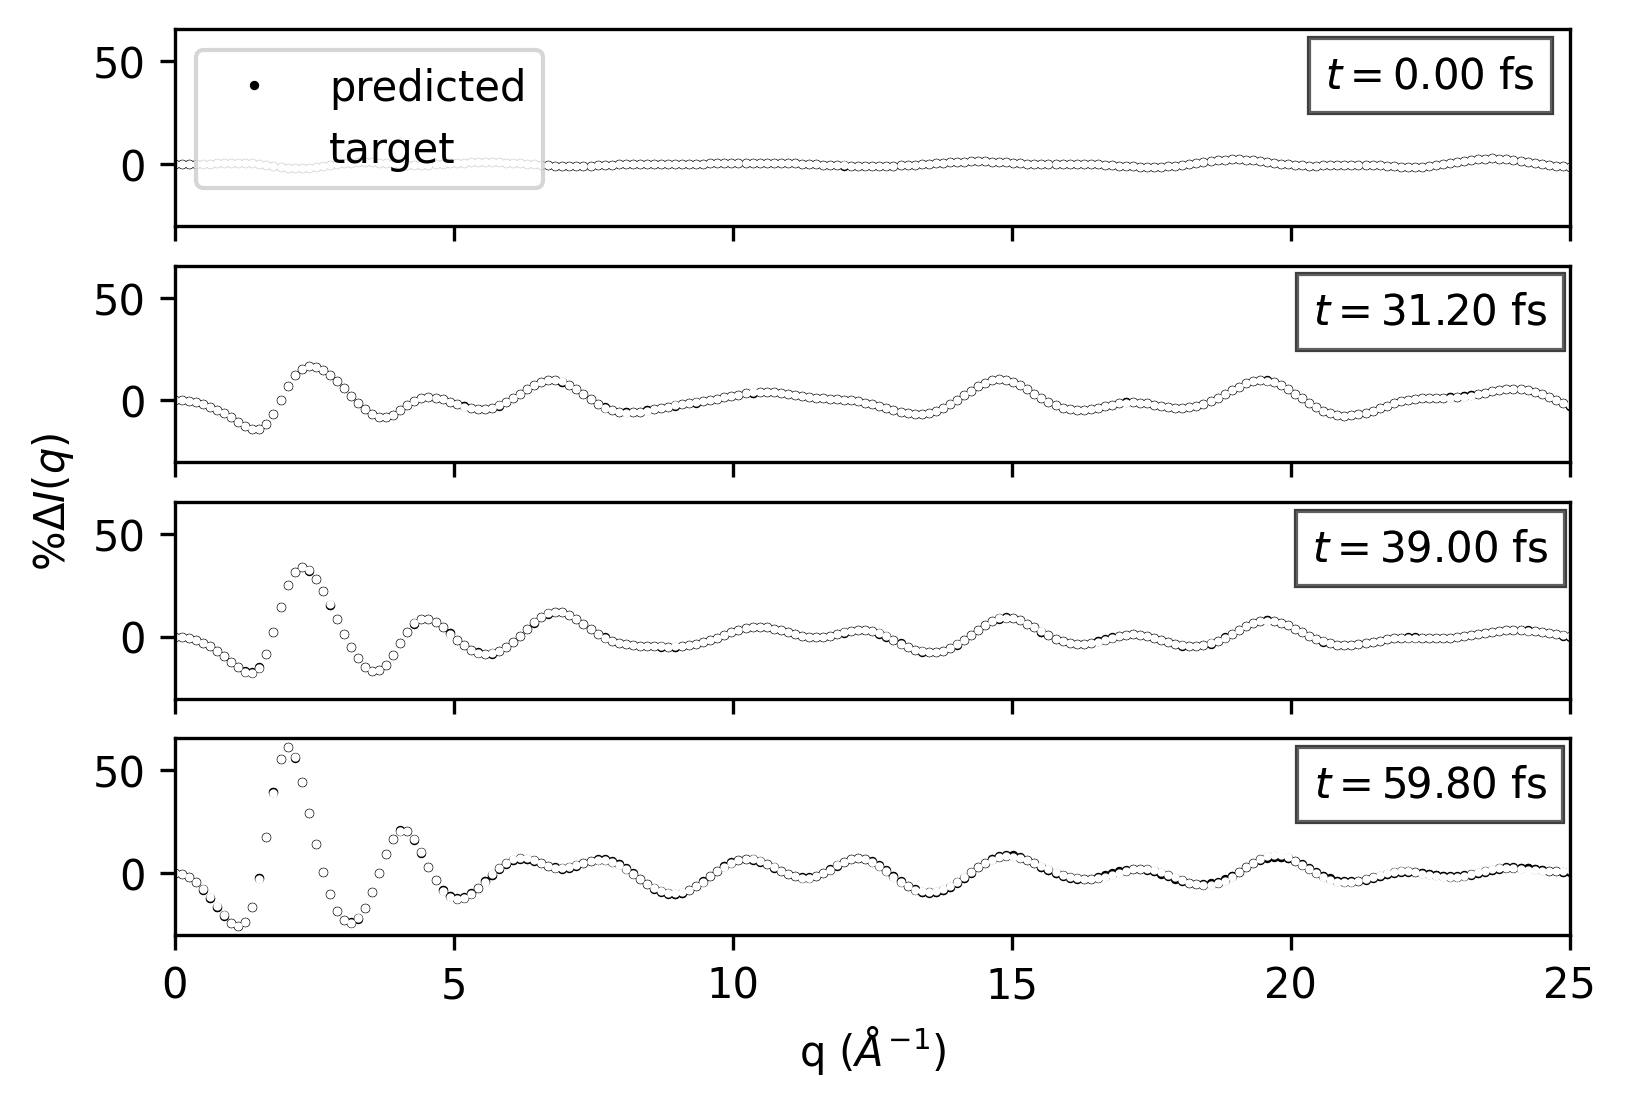
\includegraphics[width=0.8\textwidth]{lineouts.png}
	\caption{CHD x-ray scattering lineouts.}
	\end{figure}
	
	It seems like $\chi^2 \sim 0.001$ corresponds with $R_{CC}$ matching the target.
	
	\begin{figure}[H]
		\centering
		\begin{subfigure}{0.8\textwidth}
		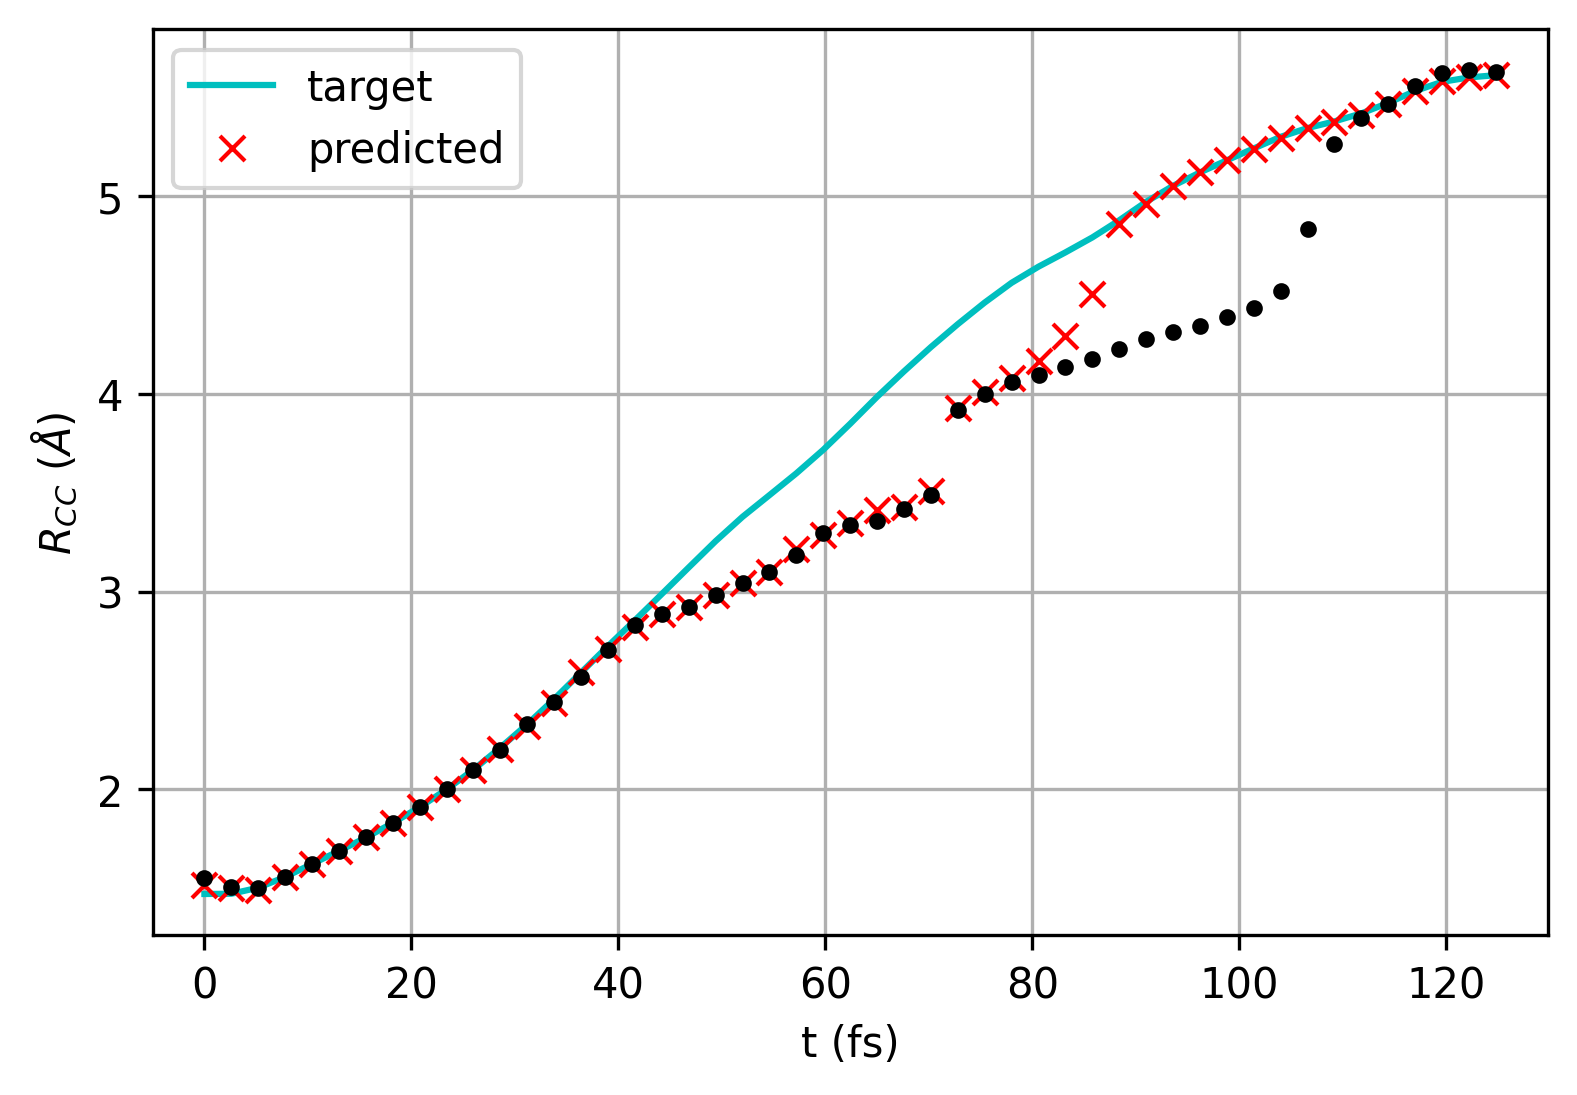
\includegraphics[width=\textwidth]{rcc_plots.png}
		\caption{Temperature cycle method: Do not restart from the starting geometry at each cycle, but start at the last geometry of the previous cycle.}
		\end{subfigure}
	\hfill
		\begin{subfigure}{0.8\textwidth}
			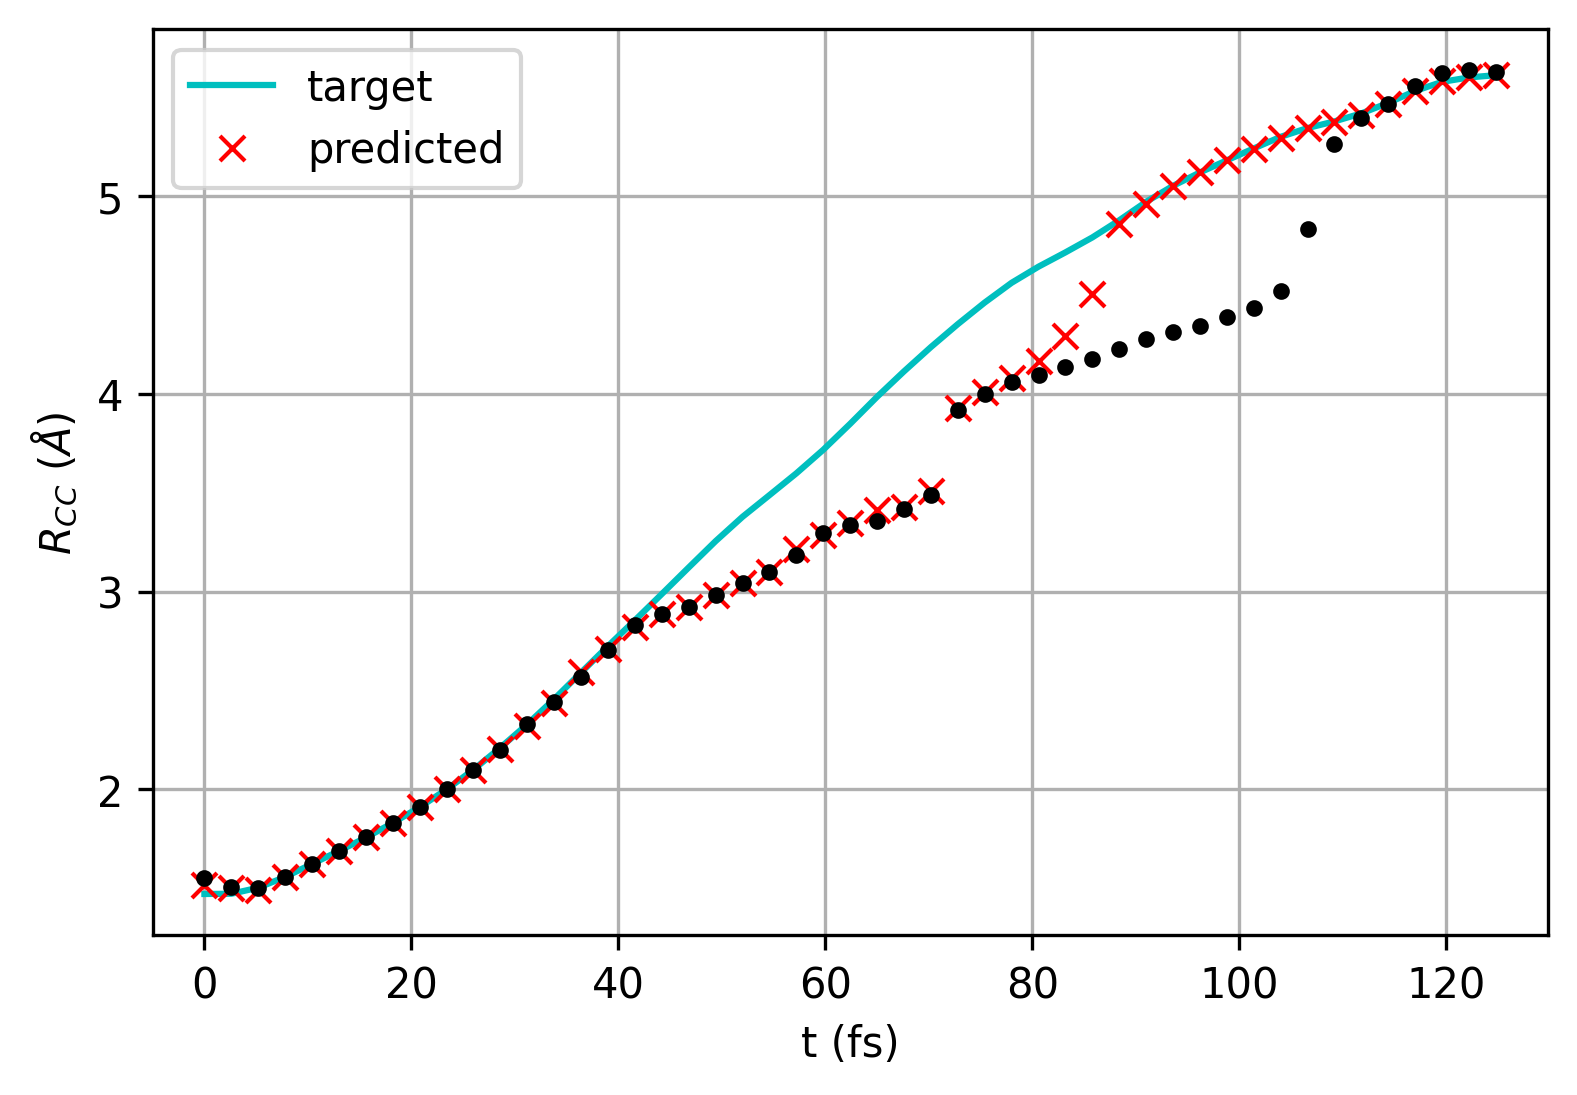
\includegraphics[width=\textwidth]{rcc_plots.png}
			\caption{Robust restart method: Restart from a slight perturbation of the starting geometry at each cycle, and use 5x the amount of steps per cycle.}
		\end{subfigure}
		\caption{CHD ring-opening C-C distance, $R_{CC}$. The target is from a surface hopping trajectory. Predictions are using $q_\textrm{max} = 25.0$ \AA$^{-1}$.}
		\label{fig:rcc_q25}
	\end{figure}

	\begin{figure}[H]
	\centering

		\begin{subfigure}{0.6\textwidth}
			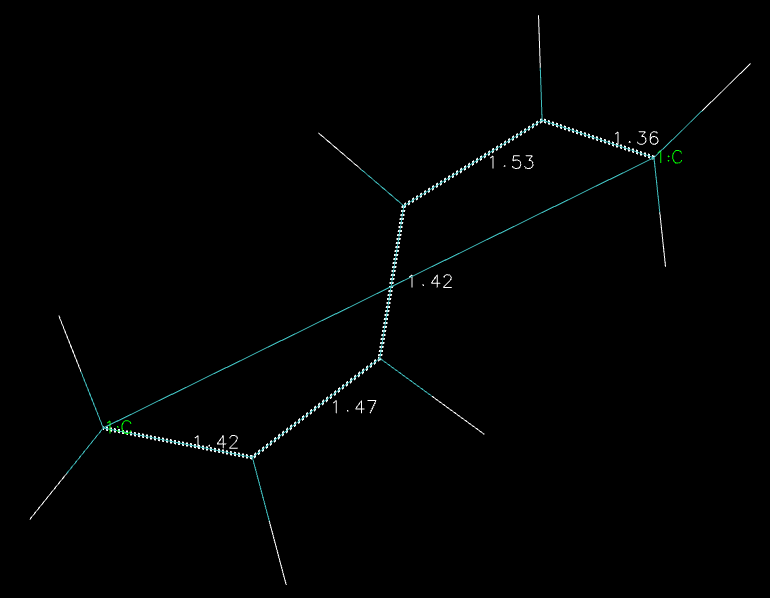
\includegraphics[width=\textwidth]{target_step48.png}
			\caption{Target.}
			\label{fig:chd_target}
		\end{subfigure}
	\hfill
		\begin{subfigure}{0.6\textwidth}
			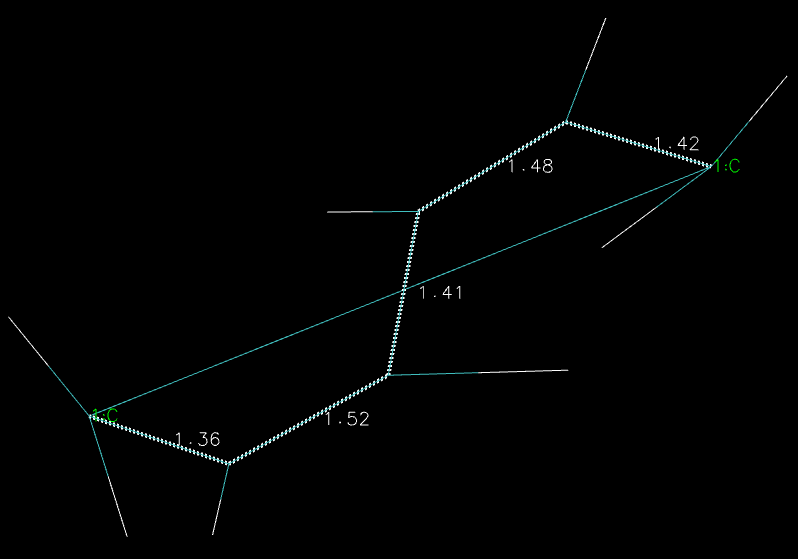
\includegraphics[width=\textwidth]{1003.png}
			\caption{Predicted.}
			\label{fig:chd_predicted}
		\end{subfigure}
	\caption{CHD target and predicted, showing all C-C bond-lengths.}
	\label{fig:figures}
	\end{figure}

\bibliographystyle{plain}
\bibliography{library}
	
\end{document}
